%!TEX root = ../template.tex
%% ====================================================================
%% Apêndice D -- Manual do dashboard
%% O corpo do manual entra como PDF incluído; o bloco \includepdf e as
%% entradas de índice são gerados por _gerador/manual_apendice.py a partir
%% de ../manual-dashboard/Manual_Dashboard_Energia_apendice.docx.
%% Não copiar metadados/09_roles_perspetivas_fontes.csv (connection strings).
%% ====================================================================

\chapter{Manual do \emph{dashboard}}
\label{app:manual}

O \emph{dashboard} descrito no Capítulo~\ref{cha:plataforma} foi entregue com
um manual, e é esse manual que se reproduz aqui. Não é um resumo escrito para
a dissertação: é o documento operacional da equipa de monitorização de
processo, mantido por ela, cuja fonte vive na pasta partilhada ao lado do
ficheiro do \emph{dashboard}. O que se segue é a versão fixa à data da
entrega --- \emph{dashboard} v22 e mapeamento mestre v22, sobre a extração do
modelo de 31 de julho de 2026.

\paragraph{Porque acompanha a dissertação.} Três razões. A primeira é de
prova: o Capítulo~\ref{cha:plataforma} afirma decisões de desenho --- os três
perímetros de consumo, a precedência entre canais, o limiar de carga por
unidade, a reta anual por unidade e vetor --- e o manual é onde essas
decisões estão escritas para quem tem de as manter, com o motivo ao lado. A
segunda é de âmbito: a plataforma só é utilizável se alguém a puder operar e
alterar sem o autor, e um manual que passe esse teste faz parte do
entregável, não é documentação acessória. A terceira é de honestidade: o
manual traz as suas próprias lacunas visíveis, e é preferível mostrá-las a
descrevê-las.

\paragraph{O que está incluído.} O corpo do manual, integral: a casca
(regras de manutenção, cobertura atual e pendências, pré-requisitos de acesso
e as duas tabelas de despacho, por papel e por sintoma); a Parte~A, que
ensina a operar --- quatro caminhos de diagnóstico, uma secção por página do
\emph{dashboard} com a respetiva captura, e os conceitos de que o operador
precisa; a Parte~B, que explica como o sistema é feito e como se muda ---
topologia, um capítulo por componente com função, interfaces, mecânica,
justificação e modos de falha, os casos de manutenção e o dicionário de dados;
e o capítulo de estado futuro. Ficam de fora os anexos da versão entregue à
refinaria: as secções-modelo para crescer o documento, o catálogo das
159 medidas com o código \gls{DAX} de cada uma, o código
\emph{Power Query} das 21 consultas e das 32 partições, e a
galeria com os 33 estados capturados. São material de referência para
quem mantém o modelo, somam mais de uma centena de páginas de código e
incorporam a correlação licenciada da metodologia de comparação externa, que
não é reproduzível aqui.

\paragraph{Como ler as marcas.} O manual assinala a laranja, com
\textsf{[POR PREENCHER: \ldots]}, aquilo que só pode ser preenchido por quem
tem acesso ao sistema: o dono do documento, o \emph{workspace} e o endereço de
produção, a hora e o responsável da atualização agendada, os destinatários de
cada ação de diagnóstico. O acesso do autor ao \emph{dashboard} terminou com o
estágio, e a alternativa --- inventar valores plausíveis --- seria pior do que
a lacuna assinalada. A vermelho, entre sinais de menor e maior, estão os
caminhos internos tornados genéricos: o servidor de ficheiros, a unidade de
rede dos planos de fabrico e a pasta do mapeamento mestre. Não há credenciais
no documento nem no código que ele reproduz; o acesso ao historiador faz-se
por uma fonte de dados configurada na máquina que atualiza o modelo. A cópia
entregue à refinaria segue com um documento de instruções que lista as duas
coisas, marca a marca.

\paragraph{O que é estado e o que é proposta.} A distinção percorre o manual e
importa para a leitura: o que o sistema cobre em julho de 2026 está na tabela
de cobertura da casca, com as pendências declaradas linha a linha, e é essa
tabela --- não a ausência de um visual --- que diz se algo devia lá estar. O
bloco de saúde das \emph{baselines} que o Capítulo~\ref{cha:discussao} propõe
a partir do diagnóstico aparece no capítulo de estado futuro do manual,
identificado como proposta não implantada. Nada do que está nas Partes~A e~B
descreve funcionalidade que não exista.

\paragraph{Correspondências com o corpo da dissertação.} A tabela de cobertura
e os modos de falha dos componentes de ingestão e mapeamento são a forma
operacional dos achados da validação descrita na
Secção~\ref{sec:validacao-dados}. A advertência de que a banda de $\pm2\hat\sigma$
vale no ano em que foi estimada, e de que a cobertura fora da amostra variou
entre 38 e 99,7\,\% conforme o par de anos, é a passagem do
diagnóstico do Capítulo~\ref{cha:diagnostico} para a linguagem de quem lê o
\emph{dashboard} todas as manhãs. E o caso de manutenção que manda validar
cada mês contra o fecho oficial, com as duas pistas de deteção rápida, é o
procedimento que a validação de julho de 2026 deixou como método.

\medskip
\noindent As páginas que se seguem são o manual tal como foi entregue. A
numeração é a dele; os capítulos e as partes estão listados no índice desta
dissertação.

\clearpage
%% GERADO por _gerador/manual_apendice.py — não editar à mão.
%% Fonte: ../manual-dashboard/Manual_Dashboard_Energia_apendice.docx
% 46 páginas; 11 entradas de índice.
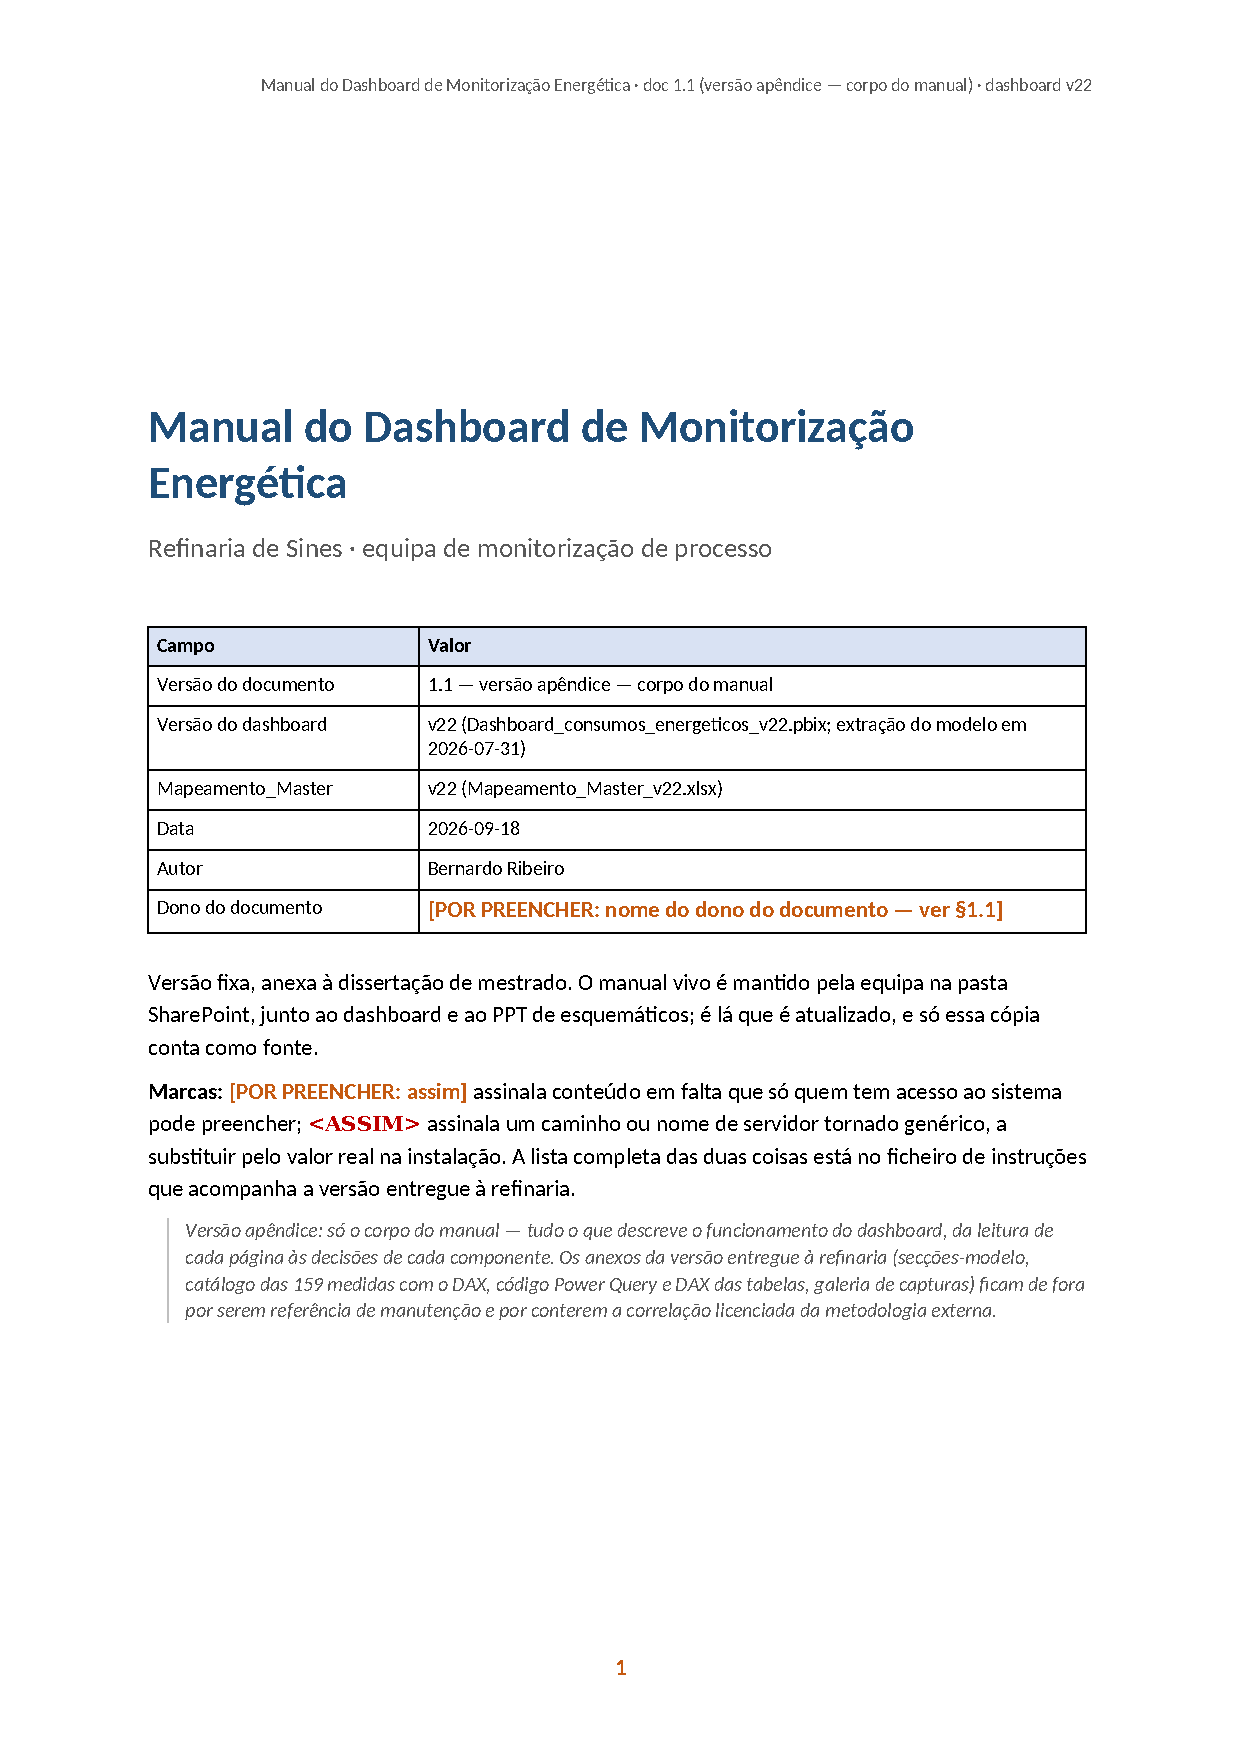
\includepdf[pages=-,scale=0.82,frame,pagecommand={\thispagestyle{plain}},
  addtotoc={
    2,section,1,{Início -- como usar este manual},man:1-in-cio-como-usar-este-manu,
    9,section,1,{Parte A -- Operar o dashboard (guia do utilizador)},man:parte-a-operar-o-dashboard-g,
    9,section,1,{Narrativa de diagnóstico},man:2-narrativa-de-diagn-stico,
    11,section,1,{Referência página a página},man:3-refer-ncia-p-gina-a-p-gina,
    15,section,1,{Conceitos para o operador},man:4-conceitos-para-o-operador,
    18,section,1,{Parte B -- Manter e estender (manual técnico)},man:parte-b-manter-e-estender-ma,
    18,section,1,{Topologia},man:5-topologia,
    19,section,1,{Componentes},man:6-componentes,
    28,section,1,{Casos de manutenção},man:7-casos-de-manuten-o,
    30,section,1,{Dicionário de dados},man:8-dicion-rio-de-dados,
    45,section,1,{Estado futuro -- roadmap e pedidos},man:9-estado-futuro-roadmap-e-pe
  }]{5-Figures/apendice-D/manual-corpo.pdf}

